\documentclass[a4paper]{article}
\usepackage[top=1in, bottom=1.25in, left=1.25in, right=1.25in]{geometry}
\usepackage{amsmath}
\usepackage{multicol}
\usepackage{graphicx}
\RequirePackage{ltxcmds}[2010/12/07]
%opening
\title{Discrete to Continuous Time}


\begin{document}

\maketitle

This block converts a signal from a discrete time signal to a continuous time signal. To do so it reads the input signal buffer value, puts it in the output signal buffer and it fills the rest of the space available for thar symbol with zeros.

\subsection*{Input Parameters}

\begin{itemize}
	\item numberOfSamplesPerSymbol 
\end{itemize}

\subsection*{Functional Description}

\subsection*{Input Signals}

\textbf{Number}: 1

\textbf{Type}: Sequence of 1's and -1's. (DiscreteTimeDiscreteAmplitude)

\subsection*{Output Signals}

\textbf{Number}: 2

\textbf{Type}: Sequence of Dirac Delta functions (ContinuousTimeDiscreteAmplitude)

\subsection*{Example}

\begin{figure}[h]
	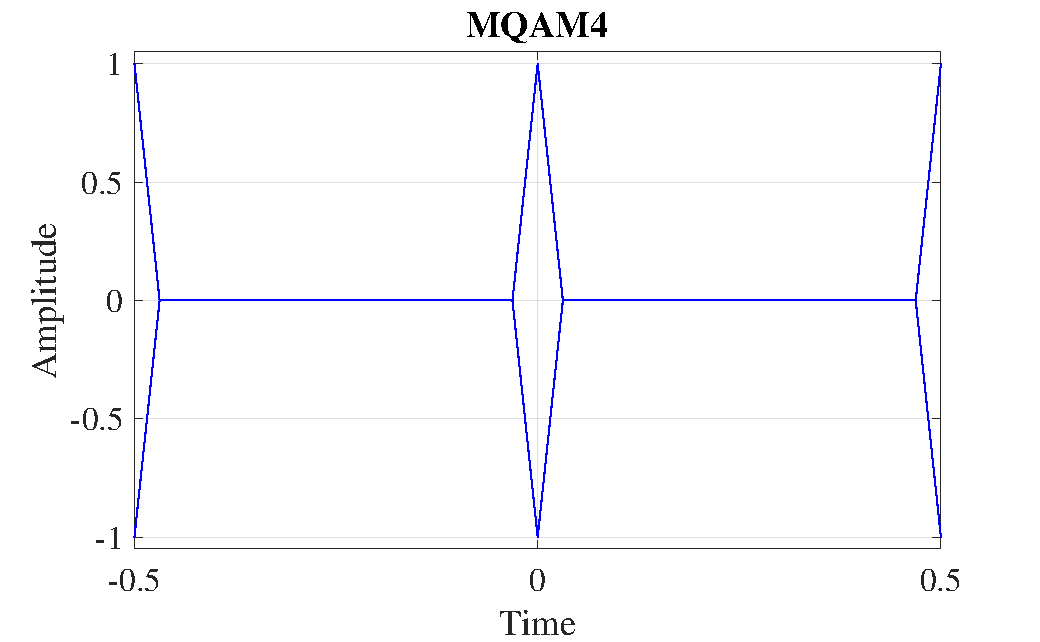
\includegraphics[width=\textwidth]{MQAM4}
\end{figure}

\subsection*{Sugestions for future improvement}

\pagebreak



\end{document}